\documentclass[10pt]{article}
\usepackage[utf8]{inputenc}
\usepackage[spanish]{babel}
\usepackage[usenames,dvipsnames,svgnames,table]{xcolor}
\usepackage{multirow}
\usepackage{diagbox}
\usepackage{booktabs}
\usepackage{anysize} 
\usepackage{hyperref}
\usepackage{helvet}
\renewcommand\refname{Referencias}
\marginsize{2cm}{2cm}{2.0cm}{2cm}
\usepackage{enumitem}
\usepackage{setspace}
\usepackage{scrextend}
\addtokomafont{labelinglabel}{\sffamily}

%% Graphics
\usepackage{graphicx}
\usepackage{color}
\usepackage{gensymb}
\usepackage{multirow}
\usepackage{caption}
\usepackage{float}


\hypersetup{
	colorlinks=true,
	linkcolor=blue,
	filecolor=magenta,
	urlcolor=cyan,
	citecolor=blue
}





\begin{document}
	\title{Fundamentos de Bases de Datos \\
		Practica 3\\ Modelado de Datos
	} 
	\author{}
	\date{12 de Marzo del 2019}
	\maketitle
	
	\section{Diagrama E/R del caso de uso}
	
	El siguiente diagrama esta basado de acuerdo a las especificaciones en el caso de uso.
	
		\begin{figure}[H]
		\centering
		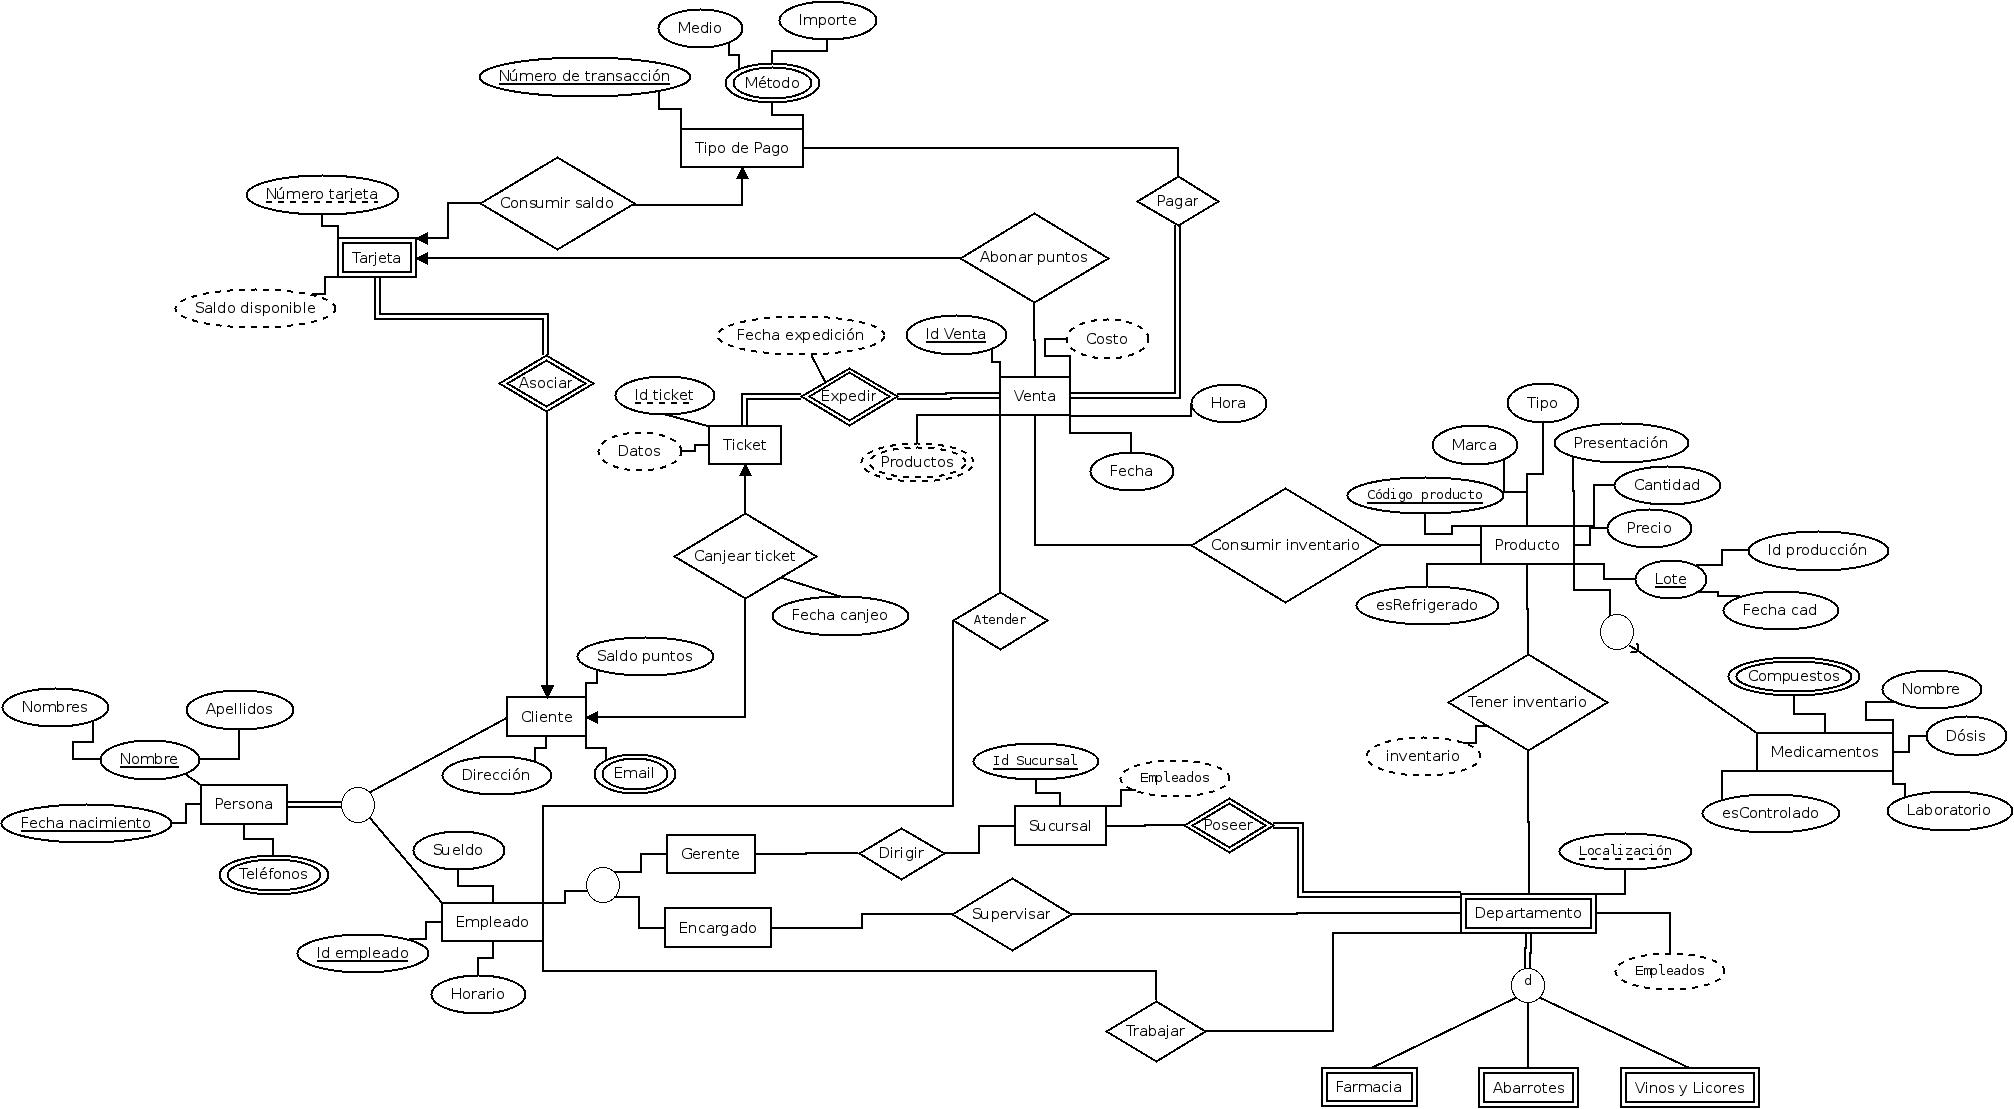
\includegraphics[width=1 \textwidth]{practica03.jpeg}
		\caption{Diagrama E-R para "\,El rey de los Abarrotes ".}
	\end{figure}


\section{Desarrollo}
Se decidió modelar el caso de uso de la siguiente manera.
\subsection{Entidades}
\begin{itemize}
	\item Fuertes
	\begin{description}[leftmargin=8em,style=nextline]
		\item [Sucursal]
		\item [Persona]
		\item [Empleado:] Es una entidad porque es necesario tener la información sobre las personas que trabajan en alguna sucursal.
		\item [Gerente]
		\item [Encargado]
		\item [Cliente]
		\item [Venta]
		\item [Ticket]
		\item [Producto]
		\item [Tipo de pago:] Esta entidad indica el tipo de pago que realiza un cliente, 
		\item [Farmacia]
		\item [Medicamentos]
		\item [Abarrotes] 
		\item [Vinos y Licores]
		
	\end{description}
	\item Débiles
	\begin{description}[leftmargin=8em,style=nextline]
		\item [Tarjeta:] Corresponde a la tarjeta digital de puntos y es una entidad débil porque debe estar asociado al id del cliente.
		\item [Departamento]
	\end{description}
\end{itemize}

\subsection{Relaciones}
\begin{itemize}
	\item
	
	\begin{description}[leftmargin=8em,style=nextline]
		\item[Trabajar]
		\item[Supervisar]  
		\item[Dirigir]
		\item[Pagar]
		\item[Abonar puntos]
		\item[Expedir]
		\item[Canjear ticket]
		\item[Consumir saldo]
		\item[Tener inventario]
		\item[Consumir inventario]
		\item[Asociar]
		\item[Poseer] 
	\end{description}
\end{itemize}
	



\section{Bitácora}
	
	\begin{labeling}{alligator}
		\item [04/03] Inicio de proyecto Categorizamos entidades (a-atributadas) y relaciones sin detalles ($\#$, part, ...). PENDIENTES: definir como representar herencia sin herencia, todo lo que falto en el modelo (detalles).
		\item [05/03] E-R Ext es válido, adecuamos ejemplos en el laboratorio. 
		\item [07/03] Definir relaciones finales, terminar diseño 'tipo de pago'.
		\item [11/03] La idea esta completa!
	\end{labeling}
	
	
	
\end{document}